\setcounter{secnumdepth}{1}
\renewcommand{\chaptername}{Rozdział}
%============================================================================================================================
%							 						Fabuła
%============================================================================================================================
\chapter{Wprowadzenie} 

\section{Fabuła}
\lhead{Rozdział 1. \emph{Fabuła}}

Celem gracza będzie przebiec jak największy dystans. Będzie to bieg astronauty przez obcą planetę na której musi zbierać bańki z tlenem oraz omijać przeszkody żeby nie zginąć. Przeszkodami takimi będą meteoryty zmniejszające poziom życia. Astronauta podczas gry będzie cały czas biec do przodu,zwalniając jedynie w przypadku niskiego poziomu życia.

\begin{wrapfigure}{left}{0.5\textwidth}
\begin{center}

\includegraphics[width=120px]{./Pictures/astro.jpg}
\end{center}
\caption{Postać astronauty }
\label{Etykieta}
\end{wrapfigure}

Poziom życia będzie ciągle spadał, i bańki z tlenem będą go zwiększać. 
Gracz będzie miał możliwość podskakiwania astronautą oraz wznoszenia się nim do góry Sporadycznie na mapie będą się pokazywać bonusy który astronauta będzie mógł zebrać (maksymalnie 3 naraz) i wykorzystać później do uzupełnienia ilości życia. Taki bonus będzie dawał także nieśmiertelność przez kilka sekund, wtedy to na brzegach ekranu pojawi się charakterystyczna obwódka. Kiedy gracz zakończy grę, wtedy jego wynik, czyli ilość przebytych metrów zapisywany będzie na liście 10 najlepszych wyników. Wyniki te będą zapisywane w osobnym pliku na dysku, tak żeby dane nie zostały stracone po wyłączeniu aplikacji. Listę najlepszych wyników będzie można obejrzeć wybierając z głównego menu pozycje „highscore”. Ze względu na fabułę z biegnącym
astronautą, oraz osadzenie zdarzeń na obcej planecie, gra została nazwa „Astro Rush”.


%============================================================================================================================
%							 						 Grafika
%============================================================================================================================
\section{Grafika}
\lhead{Rozdział 1. \emph{Grafika}}

Grafika w grze będzie się opierać o tzw. sprite. Technika ta polega na tworzeniu animacji, bądź też rysowania dużych obrazów z serii małych obrazków
które zazwyczaj są fragmentami jednej grafiki. Poszczególne klatki animacji biegu astronauty przedstawia na rysunek 2.

\begin{figure}[h]
    \centering
    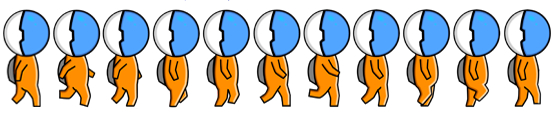
\includegraphics[width=0.8\textwidth,natwidth=410,natheight=142]{./Pictures/astroRun.jpg}
    \caption{Animacja biegu astronauty}
\end{figure}

Wszystkie animacje w grze są przechowywane w jednym głównym pliku „atlas.png”. Skąd wyświetlany jest tylko fragment odpowiadający danemu sprite-owi.
Po upływie określonego czasu następuje przejście do następnej klatki animacji, czyli zazwyczaj przesuniecie współrzędnej X o szerokość obrazka. W tym
algorytmie współrzędna Y nie zmienia się. Cały algorytm wyświetlania animacji opartej przestawia schemat 1.
Warto tutaj wspomnieć o układzie współrzędnych jaki jest używany w bibliotece SDL. Otóż punkt początkowy (0,0) znajduje się w lewym górnym
rogu, prawy górny wierzchołek to ( szerokość okna, 0 ), natomiast lewy dolny to : (0, wysokość okna ). Grafika na potrzeby gry została częściowo
stworzona w edytorze grafiki wektorowej Inkscape, który oparty jest na licencji GPL i działa pod takimi systemami operacyjnymi jak np. Windows, Linux.
Narysowanie części obrazków jako grafiki wektorowej pozwoliło zachować pełną skalowalność w dalszym procesie tworzenia grafiki. Utworzone grafiki
wektorowe były składane i poprawiane w Adobe Photoshop – bardzo rozbudowanej aplikacji do obróbki grafiki rastrowej. Photoshop jest aplikacją płatną,
jednak istnieje możliwość użycia 30 dniowej wersji Trial, co też zostało zrobione podczas tworzenia gry. W atlasie grafiki znalazły się także ikony z
kolekcji „Hand drawn icon set” które autor opublikował w internecie  na darmowej licencji.

\begin{figure}[h]
    \centering
    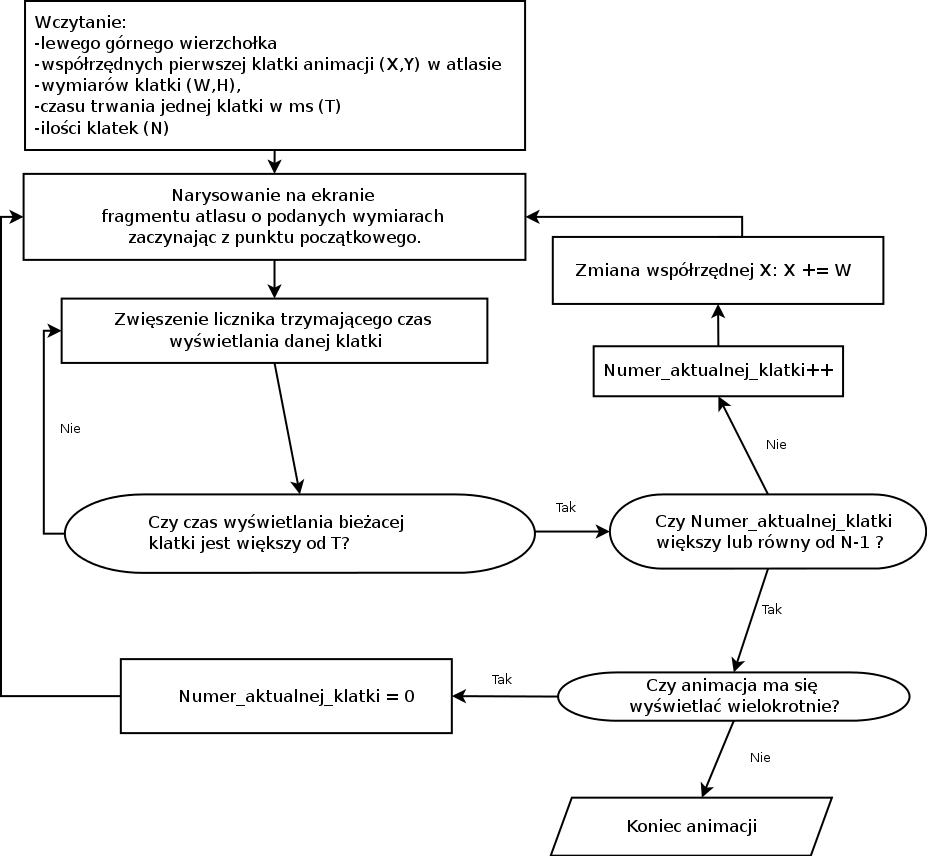
\includegraphics[width=0.8\textwidth,natwidth=410,natheight=142]{./Pictures/sprite_algorytm.png}
    \caption{Schemat wyświetlania animacji opartej o sprite}
\end{figure}

%============================================================================================================================
%							 						G++
%============================================================================================================================
\section{Użyte narzędzia}

\lhead{Rozdział 1. \emph{Użyte narzędzia}}
\subsection{Kompilator}
Do zbudowania aplikacji został wykorzystany kompilator g++ dostępny w ramach GNU GCC - zestawu kompilatorów dla popularnych języków. GCC dostępny na licencji GPL pozwala na kompilacje aplikacji napisanej w min. w Java, C/C++, Ada. Dostępny jest na wiele platform i architektur. Ponadto w systemach Linuks jest często zainstalowany domyślnie np. w Gentoo gdzie każda aplikacja jest kompilowana ze źródeł. G++ posiada kompatybilność z językiem C, dzięki czemu nie ma problemu z kompilacją programu korzystającego z biblioteki SDL, która jest napisana właśnie w C. Kompilator ten jest aplikacją konsolową, a skompilowanie zwykłego pliku źródłowego (main.cpp) do pliku wynikowego (main.bin) można wykonać za pomocą polecenia:
\begin{verbatim}
	g++ -c ./main.cpp -o main.bin
\end{verbatim}

W przypadku aplikacji składającej się z jednego pliku i nie korzystającego z żadnych bibliotek taka kompilacja wydaję się łatwa.
Kiedy natomiast mamy kilka plików do skompilowania, wtedy należy wszystkie je wpisać jako parametr, a dodatkowo trzeba ustawić 
flagi linkera, który łączy skompilowane pośrednie pliki w plik wykonywalny: (@TODO sprawdzic czy dziala)
\begin{verbatim}
	g++ -c ./main.cpp plikA.cpp plikB.cpp plikC.cpp -o main.bin -lSDL -lGL
\end{verbatim}
Projekt Astro Rush składa się z około 20 klas, wpisywanie takiego polecenia za każdym razem byłoby bardzo nie wygodne, dlatego też zostało użyte narzędzie make usprawniające budowanie gry. Zostanie ono opisane w jednym z kolejnych rozdziałów. Warto wspomnieć że g++ posiada bardzo wiele przydatnych parametrów, przy kompilacji projektu zostały wykorzystane opcje:

-Wall - włącza wszystkie ostrzeżenia przy budowaniu. 

-pedantic wlącza wszystkie ostrzeżenia związane ze standardem ISO języka C/C++

-g kompilacja z wlączonym debugiem. Do skompilowanej aplikacji dołączane są dane potrzebne do debuggowania poprzez gdb. 

-std=c++0x flaga wymusza użycie najnowszego standardu języka C++.


-O0 Określa poziom optymalizacji. Poziom 0 ustawiony domyślnie wyłącza optymalizacje, pzryśpieszając tym samym czas kompilacji. Przed udostępnieniem aplikacji użytkownikowi należy włączyć optymalizacje np. za pomocą -O3, gdzie poziom 3 jest najwyższym poziomem optymalizacji.  



%============================================================================================================================
%							 						Eclipse
%============================================================================================================================

\lhead{Rozdział 1. \emph{Użyte narzędzia}}
\subsection{Eclipse}
Środowiskiem w którym będzie powstawać aplikacja będzie Eclipse IDE (ang. Integrated Development Environment). Aplikacja została stworzona przez firmę IBM, jednak obecnie stanowi ona darmowe oprogramowanie, dostępne na licencji Eclipse Public License (EPL). Licencja ta bardzo dobrze nadaje się do wykorzystania w celach komercyjnych, dzięki czemu Eclipse jest często platforma wykorzystywaną do tworzenia oprogramowania w korporacjach. Warto wspomnieć o tym że funkcjonalność aplikacji można rozszerzać za pomocą wtyczek. Eclipse posiada nawet market ( http://marketplace.eclipse.org/ ) w którym niezależni Twórcy mogą sprzedawać stworzone przez siebie plugin-y.
Dostępne są tam zarówno płatne rozszerzenia, jak i darmowe, a samą instalacje można przeprowadzić z poziomu uruchomionej aplikacji wybierając w górnym menu Help a następnie Eclipse Marketplace.


\begin{figure}[h]
    \centering
    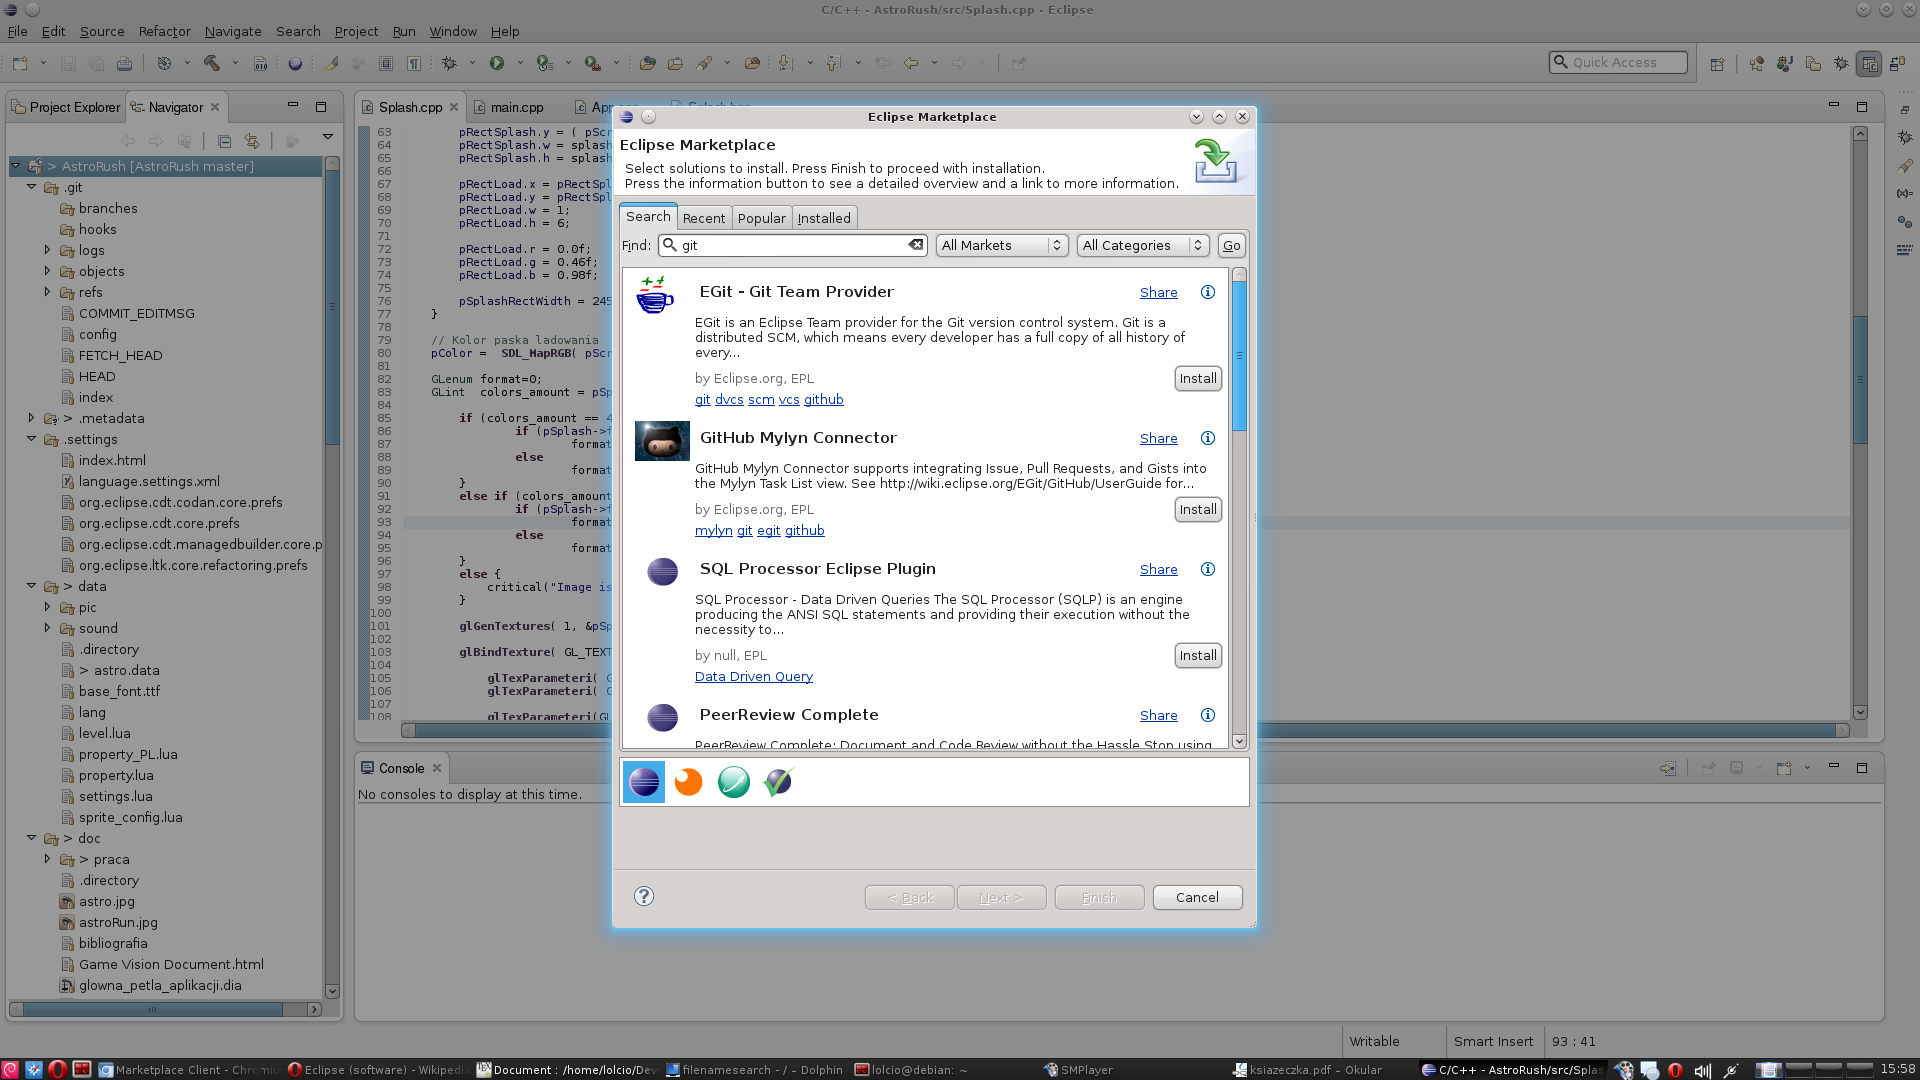
\includegraphics[width=0.8\textwidth,natwidth=480,natheight=142]{./Pictures/eclipse.png}
    \caption{Eclipse podczas instalacji wtyczki z Marketplace}
\end{figure}

Domyślnie w wersji klasycznej Eclipse możliwe jest jedynie tworzenie aplikacji w Javie, jednak instalacja wtyczki CDT, bądź też pobranie przygotowanej już odpowiedniej wersji programu pozwala na wygodne pisanie w języku C++.
Konfiguracja tego środowiska do tworzenia gry Astro Rush polegała na pobraniu z oficjalnej strony spakowanej platformy dostosowanej do języka C++, wypakowaniu jej (program wymaga do pracy zainstalowanego JRE, ponieważ napisana jest w Javie), a następnie po uruchomieniu doinstalowaniu kilku dodatkowych wtyczek które okazały się przydatne podczas tworzenia projektu np. wtyczki zapewniającej wsparcie dla repozytorium Git-a. Środowisko te posiada wbudowaną integracje z wieloma przydatnymi narzędziami, które bardzo upraszczają życie programiście np. autouzupełnienie, formatowanie kodu. Natomiast wtyczka CDT dostarczyła przy tworzeniu gry Astro Rush taki przydatnych narzędzi jak:
-Integracja Eclipse z GNU Debuggerem (w skrócie gdb). Debugger ten stworzony przez Richarda Stallmana i dostępny na licencji GPL jest aplikacją konsolową która umożliwia debuggowanie aplikacji C++ w Eclipse. Najbardziej przydatna okazała się tutaj możliwość zatrzymania programu na ustawionym breakpoincie oraz sprawdzenie stosu wywołań. Można również wykonywać kod programu krok po kroku, szukając przyczyny ewentualnych błędów. Używanie gdb z poziomu konsoli byłoby bardziej uciążliwe. 
-Integracja z Make (samo narzędzie zostanie omówione w kolejnym podrozdziale) dzięki czemu nie ma potrzeby wpisywania polecenia make w konsoli za każdym razem przy budowaniu, ale wystarczy w oknie Eclipsa wybrać cel budowania i dwa razy kliknąć w niego.

Trzeba również wspomnieć o tym że przy tworzeniu projektu został wykorzystany plugin integrujący Eclipse z programem Valgrind. 
Ta aplikacja konsolowa jest narzędziem do debugowania pamięci oraz do wykrywania wycieków pamięci. Plugin ten okazał się pomocny wielokrotnie do wyszukania miejsc w aplikacji gdzie dynamicznie przydzielana pamięć nie była zwalniania. Valgrind pozwala nawet znaleźć zmienne które nie są inicjalizowane, co pozwala uniknąć niektórych błędów związanych z tym że zmienne automatyczne zawierają po utworzeniu przypadkowe wartości z pamięci. 

W ostatniej fazie tworzenia projektu zostało wykonane profilowanie, czyli dynamiczna analiza aplikacji pozwalająca znaleźć miejsca aplikacji których wywołanie trwa najdłużej w celu ich optymalizacji. Do tego celu został wykorzystany plugin łączący Eclipse z profilerem Perf. Pozwolił on na zebranie i wyświetlenie statystyk odnośnie czasu procesora jaki jest wykorzystywany przez poszczególne funkcje, klasy w programie.

%============================================================================================================================
%					    Make jako narzędzie do automatyzacji budowania projektu
%============================================================================================================================
\subsection{Make jako narzędzie do automatyzacji budowania projektu}

Eclipse jako platforma programistyczna dedykowany jest językowi Java, a kolejne wtyczki pozwalające pisać w innych językach to tylko rozszerzenie tego środowiska Javy. Eclipse z wtyczką do języka C++ może używać programu Make, który automatyzuje budowanie projektu składającego się z wielu plików. Zostało to wykorzystane w projekcie. Ogromnym plusem takiego rozwiązania jest to żeby zbudować aplikacje u klienta nie potrzeba ściągać Eclipse-a i konfigurować projektu, ale wystarczy aplikacja make, która zajmuje niewiele miejsca na dysku i  wystarczy wykonać jedno polecenie żeby zbudować projekt. Rozwiązanie takie jest nie zależne od systemu, ponieważ make działa zarówno w systemie Windows jak i Linux. Dodatkowo bardzo łatwo się go instaluje w większości dystrybucji Linuksa. Dla dystrybucji Debian będzie to polecenie:

\begin{verbatim}
	aptitude install make
\end{verbatim}

Po uruchomienia programu make, szuka on domyślnie, o ile nie podaliśmy w parametrach innej nazwy - pliku Makefile. Plik ten opisuje zależności miedzy plikami źródłowymi, i umożliwia skompilowanie tylko tych plików które uległy zmianie od ostatniego budowania. Zdecydowanie przyśpiesza to prace nad projektem w przypadku kiedy jest potrzebne testowania poprawek na bieżąco. 

Domyślne wywołanie make bez żadnych parametrów spowoduje zawsze uruchomienie domyślnego celu budowania: all. Możliwe jest definiowania dowolnej ilości celów budowania w jednym Makefile-u. Dzięki zastosowaniu takiego podejścia nie ma potrzeby edycji Makefilu kiedy chce skompilować aplikacje np. z innymi flagami kompilatora. Wystarczy wtedy dopisać odpowiedni cel budowania i go uruchomić. W projekcie Astro Rush został dodany również cel budowania służący do czyszczenia gry z wszystkich skompilowanych źródeł oraz z linkowanej aplikacji, co okazuje się przydatne kiedy występuje potrzeba przebudowania całego projektu. Tutaj należy wspomnieć o tym że Makefile sprawdza które pliki wymagają ponownej kompilacji, i kompiluje tylko te które uległy zmianie od ostatniego budowanie. Takie podejście znacząco skraca czas który programista musi poświecić na budowaniu aplikacji. Dodatkowo make wspiera kompilacje wielowątkowa, dzięki czemu na maszynach z procesorem wielordzeniowym można wykorzystać wszystkie rdzenie, skracając jeszcze bardziej czas budowy programu. 

Napisany na potrzeby gry plik „Makefile” pokazuje również że w pliku reguł programu make można definiować swoje zmienne. Taką zmienną może być na przykład ścieżka do kompilatora, która może się zmienić w zależności od platformy. Takimi zmiennymi mogą być również flagi linkera, kompilatora, oraz lista plików źródłowych z katalogu src. Tak napisany Makefile okazał się bardzo uniwersalny i dodanie kolejnych nowych plików źródłowych wymaga jedynie dopisanie ich na listę w zmiennej Makefile-a. 

Budowanie aplikacji poprzez make bądź też podobne narzędzie o nazwie cmake jest wyjątkowo popularne w systemie Linuks i projektach napisanych w języku C/C++. Make jest nawet wykorzystywany do budowania jądra Linuksa, które składa się z milionów linii kodu ( wersja 3.2 to w przybliżeniu 15 mln ) oraz setek plików, gdzie oszczędność czasu w przypadku rekompilacji jest bardzo znacząca kiedy kompilowane są tylko te moduły które zostały zmienione. Plik Makefile w grze Astro Rush wygląda następująco:
\begingroup
\fontsize{10pt}{12pt}\selectfont
\begin{verbatim}  
CXX = g++
CFLAGS = -Wall -pedantic -g -std=c++0x -I ./include -O0 -c

# flagi linkera
LIBS = -lGL -lGLU -lSDL -lSDL_mixer -lSDL_ttf -lSDL_image -lluabind -llua5.1

# lista plikow źródłowych do kompilacji
SOURCES = src/main.cpp src/App.cpp src/Property.cpp src/Resource.cpp 

# jak maja się nazywać skompilowanie pliki cpp
OBJECTS=$(SOURCES:.cpp=.o)

# nazwa pliku wynikowego
EXECUTABLE = AstroRush.bin

# domyslny cel dla wywolania make bez argumentu, czyli zbudowanie projektu
all: $(SOURCES) $(EXECUTABLE)

# linkowanie aplikacji
$(EXECUTABLE): $(OBJECTS)
	 @echo "\n ---- Linkowanie ---- "
	 $(CC) $(OBJECTS) -o $(EXECUTABLE) $(LIBS)

#kompilowanie plikow cpp
.cpp.o:
	 @$(CXX) $(CFLAGS) $< -o $@

# czyszczenie aplikacji przed zbudowaniem  
clean:
	rm -rf ./src/*.o
	rm ./AstroRush.bin 

\end{verbatim}  
\endgroup

%============================================================================================================================
%														Git
%============================================================================================================================

\subsection{Git - system kontroli wersji}

Projekt Astro Rush nie wydaje się zbyt duży biorąc pod uwagę fakt że nie przekroczył 10 tysięcy linii kodu. Jednak zawsze warto mieć jakąś kopie na repozytorium oraz ewentualnie możliwość poprzez historie  zmian przywrócenie jakiś fragmentów kodu. Narzędziem które okazało się tutaj pomocne jest rozproszony system kontroli wersji – git. Darmowe oprogramowanie stworzone przez Linusa Torvaldsa do zarządzania kodem jądra Linuksa. Git w założeniu ma być pomocny w pracy zespołowej nad dużymi projektami, jednak w przypadku tak małego projektu jak Astro Rush również okazał się pomocny. Git jest również narzędziem wieloplatformowym, chodź pod systemem Windows jego klient jest on wolniejszy niż na Linuksie.

\begin{figure}[h]
    \centering
    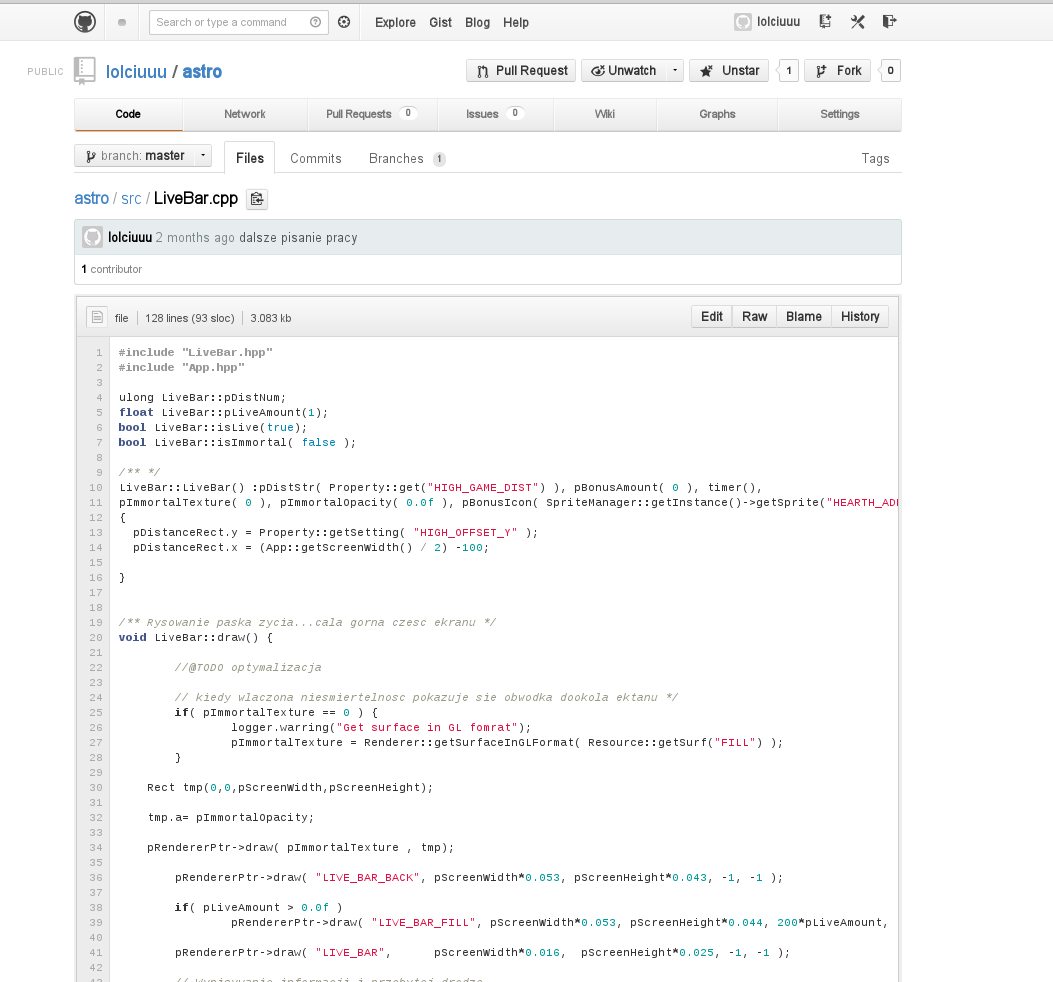
\includegraphics[width=0.8\textwidth,natwidth=490,natheight=142]{./Pictures/git.png}
    \caption{Portal github.com. Podgląd pliku źródłowego. }
\end{figure}

Przy tworzeniu aplikacji został wykorzystany serwis hostujący gita: https://github.com. Portal posiada wiele funkcji wspomagających pracę zespołową nad projektem. Pozwala między innymi na edycję plików źródłowych bezpośrednio na serwerze, przeglądanie i porównywanie zmian w plikach. Dzięki czemu łatwo można sprawdzić co było w poprzedniej wersji pliku, oraz kto wysłał zmiany (ang.commit) na serwer. Github dostarcza statystyk na temat projektu np. wykres jak zmieniała się ilość kodu wraz z kolejnymi wysłanymi wersjami na serwer. Ponadto można tworzyć na serwerze dokumentacje do aplikacji (tzw. Wiki) którą następnie użytkownik może przeglądać przez przeglądarkę, bez potrzeby ściągania na dysk. Hosting dla aplikacji open source jest darmowy, jednak w takim przypadku repozytorium z kodem jest publiczne. Oznacza to że każdy może sobie ściągnąć projekt jednym poleceniem:

\begin{verbatim}
	git clone git://github.com/lolciuuu/astro.git
\end{verbatim}

Analogicznie z poziomu konsoli można później wysyłać zmiany na serwer (o ile dany użytkownik został dodany na listę osób które mogą zmieniać pliki na serwerze ), bądź też pobierać zmiany wysłanych przez innych użytkowników. Warto wspomnieć o tym że serwis github mimo tego że powstał dość nie dawno bo w 2008, ma już 2 miliony repozytoriów. 

Git w środowisku Linuks jest narzędziem konsolowym (W systemie Debian wystarczy zainstalować pakiet o takie samej nazwie), jednak w ramach ułatwienia podczas tworzenia aplikacji została wykorzystana wtyczka do Eclipse która pozwala w łatwy sposób synchronizować projekt który znajduje się na dysku lokalnie z tym co jest na repozytorium, oraz wysyłanie zmian na serwer. Dzięki wtyczce do tej podczas tworzenia projektu nie było potrzeby wydawać poleceń z poziomu konsoli, wszystko można wykonać z poziomu GUI.


\section{OpenGL jako silnik grafiki}
\lhead{Rozdział 1. \emph{OpenGL jako silnik grafiki}}

%============================================================================================================================
%											 Czym jest OpenGL
%============================================================================================================================
\subsection{Czym jest OpenGL}
Open Graphics Library (w skrócie OpenGL) jest niskopoziomową biblioteką  graficzną 3D. Kompatybilny jest on z większością liczących się systemów
operacyjnych, został on także zaimplemtowany na urządzeniach mobilnych, przykładem może być tutaj JOGL, czyli Java-owa wersja OpenGL-a której można
używać na urządzeniach z systemem Android. OpenGL jest często wykorzystywany jako podstawowe API przy tworzeniu silników do gier 3D przykładem może
być tutaj choćby nawet silnik ID tech znany min. z serii gier Quake . Mimo że OpenGL jest przystosowany do pracy z grafiką trójwymiarową to doskonale
można go wykorzystać do grafiki 2D, tak jak to miało miejsce w grze Astro Rush. OpenGL posłużył do wyświetlania tekstur na ekranie, co odbywało się
zdecydowanie szybciej niż poprzez funkcje do rysowania z biblioteki SDL.  Różnica w szybkości renderowania wynosiła około 20 fps-ów na sekundę na
laptopie hp550 z procesorem dual core 1.4 ghz. OpenGL dostarcza także takich zaawansowanych elementów jak obsługa cieni oraz oświetlenia, jednak z
racji wykorzystania grafiki 2D nie znalazło to zastosowania w projekcie.
	W bardzo łatwy sposób można połączyć SDL-a i OpenGL-a.
W SDL podstawowym elementem graficznym na którym odbywa się rysowanie jest powierzchnia (ang. surface). Podczas inicjowania biblioteki SDL tworzona
jest główna powierzchnia na której następnie będzie się odbywać rysowanie ( często też nazywane w grafice 2D „blitowaniem” ). Podczas inicjowania
głównej powierzchni ekranu żeby używać do renderowania OpenGL-a wystarczy poprzez funkcje SDL\_SetVideoMode podać flagę SDL\_OPENGL. Trzeba jeszcze
pamiętać żeby po każdym rysowaniu wywołać funkcję: SDL\_GL\_SwapBuffers() która wysyła bufor ramki do rysowania na ekranie.


%============================================================================================================================
%							 Wykorzystanie OpenGL do renderowania grafiki w grze
%============================================================================================================================
\subsection{Wykorzystanie OpenGL do renderowania grafiki w grze}
SDL posiada rozszerzenie SDL\_image które umożliwia obsługę różnych formatów grafiki (w grze zostały wykorzystane pliki graficzne o rozszerzeniach png oraz jpeg). Pozwala one w łatwy sposób wczytać plik z dysku poprzez funkcje SDL\_Surface *IMG\_Load(const char *file) , która zwraca surface z
wczytanym obrazkiem. SDL\_Surface jest strukturą w której znajduje się wskaźnik do pamięci gdzie znajduje się wczytana z dysku grafika. Ten adres (
„void* pixels” ) należy przekazać jedynie do OpenGL-a podczas tworzenia tekstury.
Można w ten sposób rysować nie tylko pliki graficzne wczytane z dysku ale również obiekty graficzne utworzone w aplikacji. Taka sytuacja ma miejsce w
przypadku renderowania napisów, gdzie jest tworzony surface z napisem, i następnie rysowany za pomocą OpenGL-a. W aplikacji proste prymitywy graficzne
jak prostokąty wypełnione kolorem są rysowane również za pomocą API OpenGL-a.


%============================================================================================================================
%											Skrypty w języku Lua
%============================================================================================================================
\section{Skrypty w języku Lua}
\lhead{Rozdział 1. \emph{Skrypty w języku Lua}}
Lua jest lekkim językiem skryptowym zaprojektowanym do rozszerzania możliwości innych aplikacji. Został on zaimplementowany w języku C zgodnie ze standardem ANSI, zapewnia mu to przenośność na wiele platform. Najważniejszym cechami tego języka jest to że jest dynamicznie typowany, oraz obiektowy. Jest on wykorzystywany zarówno do tworzenia rozszerzeń do różnych aplikacji, co często nazywane jest skryptowaniem (ang.scripting) oraz jako samodzielny język, w którym skrypty będą wykonywane poprzez maszynę wirtualną Lua. Samo skryptowanie wiąże się z ideą programowania sterowanego danymi (ang. data driven development).
Podejście te zakłada że wszelkie stałe kontrolujące zachowanie programu oraz wybrane elementy logiki powinny być zdefiniowane poza program. W aplikacji skrypty Lua są wykorzystywane do przechowywanie wszystkich ustawień, oraz obliczania pewnych wartości 
już w czasie działania aplikacji.Przykładowo rozmiar gracza jest obliczany na poziomie skryptu przy wykorzystaniu ustawionych podczas działania gry zmiennych z rozmiarami ekranu. 

\begin{figure}[h]
    \centering
    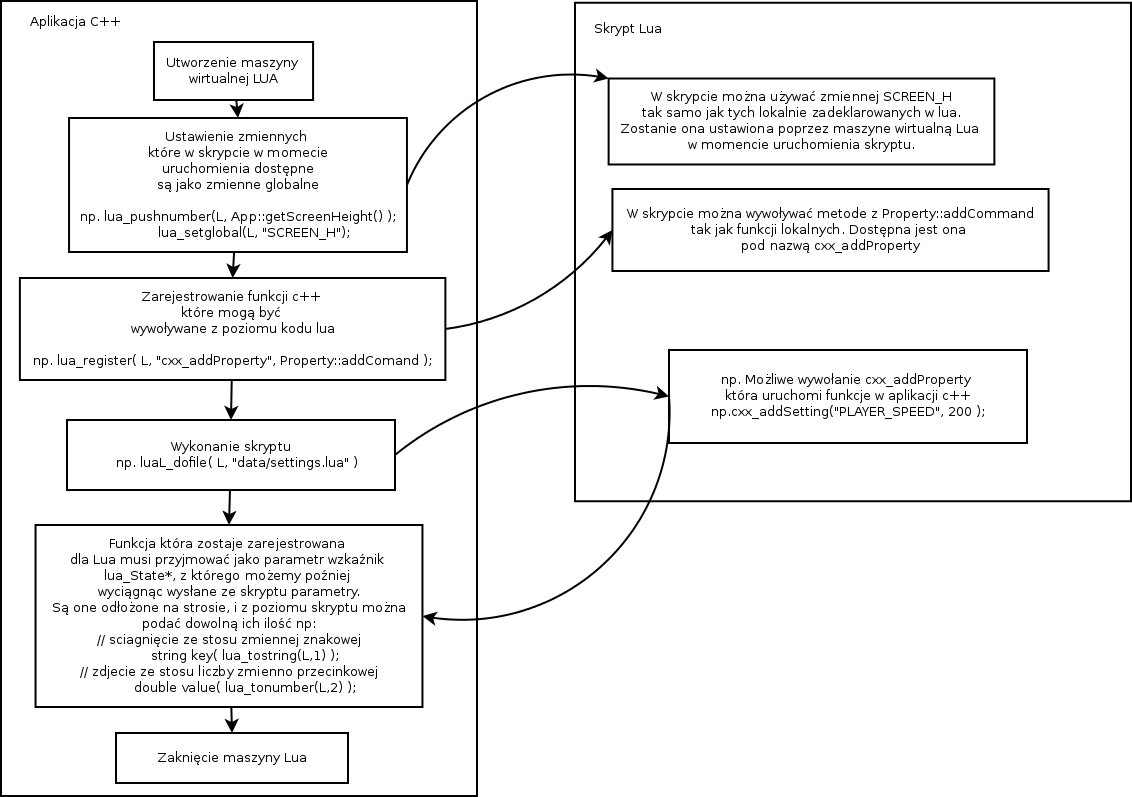
\includegraphics[width=0.8\textwidth,natwidth=410,natheight=142]{./Pictures/lua_skrypty.png}
    \caption{Przepływ danych między aplikacją C++ a skryptem Lua}
\end{figure}

Powyższy rysunek pokazuje przykładowy przepływ danych między aplikacją C++ a skryptem Lua. Wykorzystane tu zostało wywołanie funkcji C++ z poziomu skryptu, aczkolwiek w drugą stronę ten mechanizm również działa. To znaczy z poziomu C++ można wykonać funkcje Lua. Lua została wykorzystana do internacjonalizacji aplikacji. Podobnie jak to jest wykorzystywane w aplikacjach webowych w języku Java, gdzie wszystkie komunikaty są przechowywane w plikach properties. Podczas uruchamiania aplikacji zostaje odczytany odpowiedni plik dla danego języka. Cały proces ilustruje rysunek 5. W rezultacie takiej budowy aplikacja może działać z dowolnym językiem. Podczas tworzenia zostały napisane komunikaty zarówno polskie jak i angielskie.


%============================================================================================================================
%											SDL
%============================================================================================================================
\section{Wprowadzenie do biblioteki SDL}
\lhead{Rozdział 1. \emph{Wprowadzenie do biblioteki SDL}}
Rozdział ten będzie zawierał wprowadzenie do tworzenia aplikacji z wykorzystaniem biblioteki SDL, nie będzie tu poruszony temat instalacji tej biblioteki. Zagadnienie te będzie znajdować się w rozdziale dotyczącym kompilacji projektu w systemie linuks. 

Simple Direct Media Layer jest biblioteką ułatwiającą tworzenie gier komputerowych, oraz różnych aplikacji multimedialnych. Umożliwia ona stworzenie okna, oraz zarządzanie nim. Dodatkowo zapewnia obsługę zdarzeń związanych z klawiaturą, myszą oraz joystickiem. Możliwa jest nawet obsługa CD-ROM-u za pomocą tego API. Największą zaletą obok dużej funkjonalności jest prostota aplikacji pisanej z wykorzystaniem tej biblioteki. Najprostszy program może wyglądać następująo:

Tak napisany program można skompilować za pomocą kompilatora gcc z poziomu linuksowej konsoli za pomocą polecenia:

Aplikacja po uruchomieniu utrzowy okno które zostanie natychmiast zamknięte. Takie działanie aplikacji jest mało przydatnego, dlatego też konieczna jest pętla w której będzie odbywać się praca całego programu. Program wykorzystujący taką pętle może wyglądać nastepująco:
kod kod kod 

(Opis oblugi zdarzen)

SDL dostarcza również obsługę wielowątkowości oraz timerów. Dzięki czemu nie potrzebna była w projekcie żadna dodatkowa biblioteka która umożliwiała by utworzenie timera. (opis timerow)

%============================================================================================================================
%											Obsługa czcionek
%============================================================================================================================
\section{Obsługa czcionek w SDL}
\lhead{Rozdział 1. \emph{Obsługa czcionek w SDL}}
W projekcie została wykorzystana biblioteka SDL\_ttf pozwalająca używać w aplikacji czcionek w formacie True Type. Format ten stworzony przez firmę Apple przechowuje kształty poszczególnych liter jako krzywe Beziera, i jest on obsługiwany przez większość platform. Na Linuksie jest on bardzo powszechnym formatem do obsługi czcionek, dodatkowym plusem jest ogromna ilość czcionek na darmowych licencjach. W grze została wykorzystana czcionka "Ubuntu" udostępniona za darmo, i będąca domyślną czcionką w dystrybucji Linuksa o tej samem nazwie. Plik z taką czcionką (standardowo o rozszerzeniu *.ttf) jest wczytywany podczas uruchamiania aplikacji, następnie poprzez wywołania funkcji z biblioteki SDL\_ttf np. TTF\_RenderUTF\_Blended zostaje utworzona powierzchnia na której narysowany jest napis o podanej treści, kolorze oraz rozmiarze. 

Niestety powierzchnia taka jest zwracana jako wskaźnik na strukturę SDL\_Surface, przez co konieczna jest konwersja na format obsługiwany przez OpenGL-a. Niedogodność taka nie występowałaby gdyby do renderowania było wykorzystywane API biblioteki SDL. Identyczny problem występuje również przy renderowaniu innych elementów graficznych które są ładowane z dysku i zwracane jako SDL\_Surface* (Wczytywanie takie realizowane jest poprzez kolejną bibliotekę będącą uzupełnieniem SDL-a: SDL\_image. Służy ona do wczytywania plików graficznych w takich formatach jak np. JPEG, PNG, TIFF. W aplikacji wykorzystana jest tylko jedna funkcja 
z tej biblioteki stąd też nie będzie ona szerzej omawiana).

Sama konwersja SDL\_Surface* na GLuint to wygenerowanie tekstury w standardowy dla OpenGL-a sposób, wykorzystując przy tym pole pixels ze struktury SDL\_Surface, które jest adresem pod którym przechowywane są poszczególne piksele obrazka. W uproszczeniu funkcja realizująca taką konwersje w grze wygląda następująco:

\begingroup
\fontsize{10pt}{12pt}\selectfont
\begin{verbatim}  
void RendererGL::create_gl(SDL_Surface * surf, GLuint * tex )
{
 
   /** ...tutaj określenie ilości kolorów i formatu */
  
    glGenTextures( 1, tex );
    glBindTexture( GL_TEXTURE_2D, *tex );

    /** ...tutaj ustawienia parametrów tekstury */

    glTexImage2D( GL_TEXTURE_2D, 0, colors_amount,
    			  	surf->w, surf->h, 0, format, 
    			 	 GL_UNSIGNED_BYTE, surf->pixels );
}
\end{verbatim}
\endgroup

Warto wspomnieć że biblioteka SDL\_ttf pozwala renderować napisy z polskimi znakami, o ile takie występują w wczytanej czcionce. Ponadto SDL\_ttf dostępny jest podobnie jak SDL na darmowej licencji zlib, i jest wieloplatformowy jak wszystkie wtyczki do SDL-a. W niektórych dystrybucjach zainstalowanie tej biblioteki, oraz innych wspomnianych bibliotek rozszerzających SDL-a sprowadza się do wykonania jednego polecenia- zainstalowania pakietu z repozytorium. Dla dystrybucji Debian oraz jego pochodnych będzie to polecenie:
\begin{verbatim}
apt-get install libsdl-ttf2.0-dev 
\end{verbatim}